%-------------------------------------------------------------------------------
%-------------------------------------------------------------------------------
\chapter{Variables}
%-------------------------------------------------------------------------------
%-------------------------------------------------------------------------------
\thispagestyle{empty}
%-------------------------------------------------------------------------------
%-------------------------------------------------------------------------------
\begin{abstract}Dans ce chapitres nous allons introduire l'affectation. Cette instruction est très importante car elle permet de dépasser la simple machine à calculer : un ordinateur calcule, certes, mais surtout garde en mémoire le résultat calculé. L'affectation établit la connexion entre les {\bf expressions}, c'est-à-dire les calculs et les {\bf variables}. Ces deux notions sont interconnectées :
\begin{itemize}
	\item les variables mémorisent le résultat d'une expression
	\item les expressions utilisent les valeurs des variables.
\end{itemize}
\end{abstract}
%-------------------------------------------------------------------------------
%-------------------------------------------------------------------------------
\section{Variables}
%-------------------------------------------------------------------------------
%-------------------------------------------------------------------------------
L'essentiel du travail effectué par un programme d'ordinateur consiste à  manipuler des données. Ces données peuvent être très diverses, mais dans la mémoire de l'ordinateur elles se ramènent toujours en définitive à  une suite finie de bits (symboles que l’on représente par 0 ou 1) qui est stockée dans la mémoire.  Pour pouvoir accéder aux données,  il suffit de se souvenir à quelle adresse est stockée la valeur de la donnée. Cependant il est plus simple d'associer un nom à une adresse ce qui revient, pour l'utilisateur, à associer une valeur à un nom.

L'association d'une valeur à un nom se fait par l'affectation.

%-------------------------------------------------------------------------------
\begin{minipage}[b]{0.75\textwidth}
Ceci se note, en python, \Type{nom\_de\_variable = x}.

On sera vigilant sur le fait que le \type{=} de Python n'est pas l'égalité classique ;
\type{x = 4} devrait se lire {\it la variable \type{x} prend la valeur 4} et non pas {\it x égale 4}. 

D'autres langages on une écriture plus explicite :

\type{x := 4} ou \type{x <- 4}

On remarque de plus que ce signe $=$ {\bf n'est pas symétrique} : 

\type{x = 2} a un sens mais \type{2 = x} n'en a pas,

\type{a = b} donne à la variable $a$ la valeur de $b$, tandis que \type{b = a} modifie la valeur de $b$ sans changer celle de $a$.

\end{minipage}
\hspace*{0.5cm}
\begin{minipage}[t]{0.15\textwidth}
\begin{center}
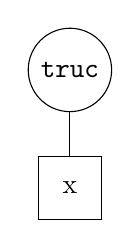
\begin{tikzpicture}
 \tikzstyle{every node}=[circle,draw,minimum size =8mm]
 \tikzstyle{level 1}=[sibling distance = 7cm]
 \node {\tt truc}
      child {node[rectangle]{x}};
\end{tikzpicture}
\end{center}
\end{minipage}
%-------------------------------------------------------------------------------
%-------------------------------------------------------------------------------
\subsection{Noms de variables}
%-------------------------------------------------------------------------------
Pour l'utilisateur une variable est d'abord un nom : les noms de variables sont des noms que vous choisissez vous-même assez librement. 

La majorité des langages ont les mêmes règles pour la création des noms de variables. 
%-------------------------------------------------------------------------------
\begin{itemize}
\item Un nom de variable est une séquence de lettres (a \dots z , A \dots Z), de chiffres (0 \dots 9) et du caractère \_ (underscore). Elle doit toujours commencer par une lettre.
\item La casse est significative (les caractères majuscules et minuscules sont distingués).

\item Il existe une liste de mots clés réservés qui ne peuvent pas être employés comme noms de variables.
Dans le cas de Python il s'agit de 

%-------------------------------------------------------------------------------
\begin{tabular}{p{16mm}p{16mm}p{16mm}p{16mm}p{16mm}p{16mm}p{16mm}}
and & as & assert & break &  class &  continue & def\\
del & elif & else & except & False & finally & for\\
from & global & if & import & in & is & lambda\\
None & nonlocal & not & or & pass & raise & return\\
True & try & while & with & yield\\
\end{tabular}

%-------------------------------------------------------------------------------
\end{itemize}
%-------------------------------------------------------------------------------
Il y a, de plus, quelques usages qu'il est recommandé de respecter.
%-------------------------------------------------------------------------------
\begin{itemize}
%-------------------------------------------------------------------------------
\item Choisissez de préférence des noms aussi explicites que possible, de manière à exprimer clairement ce que la variable est sensée contenir. 

Par exemple si on a besoin d'un majorant, d'un minorant et d'une moyenne il vaut mieux éviter des les appeler \type{m1}, \type{m2} et \type{m3}, on ne saura pas vraiment à quoi ils correspondent.
Il vaudrait mieux utiliser simplement \type{majorant}, \type{minorant} et \type{moyenne}.

Par contre \type{majorant\_des\_termes\_de\_la\_suite} est sans doute un peu excessif.

\item Prenez l'habitude d'écrire l'essentiel des noms de variables en caractères minuscules (y compris la première lettre). 

\item Les majuscules ou le symbole \_ permettent de découper le nom : 

\type{premierTerme} ou \type{premier\_terme}.

\end{itemize}
%-------------------------------------------------------------------------------
\subsection{Expressions}
%-------------------------------------------------------------------------------
%-------------------------------------------------------------------------------
La valeur que prend une variable peut être donnée explicitement : \type{g = 9.81}

Le plus souvent ce sera le résultat d'un calcul, c'est la valeur d'une expression : \type{somme = 2 + 3}.
%-------------------------------------------------------------------------------
\begin{defin}
Une  expression est une portion de code que l'interpréteur Python peut évaluer pour obtenir une valeur.
\end{defin}
%-------------------------------------------------------------------------------
L'affectation se fait en 3 étapes successives. 
%-------------------------------------------------------------------------------
\begin{itemize}
\item L'expression est évaluée, le résultat est stocké à une adresse \type{ad}.
\item Un nouveau nom de variable est défini (même s'il existait déjà avant)
\item \type{ad} est liée au nom de la variable.
\end{itemize}
%-------------------------------------------------------------------------------
Une expression peut utiliser des variables déjà définies : lors de l'affectation la valeur {\bf à l'instant du calcul} de la variable est utilisée, le résultat ne sera pas mis à jour si la variable est associée plus tard à une autre valeur.
%-------------------------------------------------------------------------------
Par exemple l'instruction \type{a = 2 + b} :
%-------------------------------------------------------------------------------
\begin{enumerate}
    \item cherche la valeur de \type{b}, par exemple 3,
\item calcule 2 + b, ce qui donne l'entier 5,
\item réserve de la place en mémoire pour un entier,
\item y stocke l'entier 5,
\item associe le nom de variable \type{a} à cette adresse.
\end{enumerate}
%-------------------------------------------------------------------------------
La temporalité permet d'écrire des instructions de la forme \type{i = i + 1} : l'ancienne valeur de \type{i} est lue, on lui ajoute 1 et on affecte cette nouvelle valeur à la variable de nom \type{i}. L'ancienne valeur est perdue.
%-------------------------------------------------------------------------------
%-------------------------------------------------------------------------------
\subsection{Une bonne pratique}
%-------------------------------------------------------------------------------
%-------------------------------------------------------------------------------
On peut s'étonner du premier exemple donné ci-dessus : \type{g = 9.81}. Pourquoi créer une variable pour une valeur fixée ? En fait il est recommandé de systématiquement affecter à une variable les valeurs numériques que l'on emploie. La avantages sont multiples.
\begin{itemize}
    \item {\bf La lisibilité} : dans les expression, les valeurs numériques ne donnent pas le sens de ce qu'elles représentent, une variable au nom bien choisi aide à la compréhension.
    \item {\bf La cohérence} : quand une même valeur est utilisée plusieurs fois, il est important que la valeur écrite soit la même à chaque occurrence, nous sommes capables de nous tromper.
    \item {\bf La variabilité} :  si on veut modifier la valeur utilisée, modifier la variable associée est beaucoup plus simple que de repérer toutes ses apparitions et de les changer.
\end{itemize}
%-------------------------------------------------------------------------------
\newpage
%-------------------------------------------------------------------------------
\section{Opérations de base}
%-------------------------------------------------------------------------------
%-------------------------------------------------------------------------------
\subsection{Entiers}
%-------------------------------------------------------------------------------
%-------------------------------------------------------------------------------
Les opérations sur les entier sont, en Python,
%-------------------------------------------------------------------------------
\begin{itemize}
\item +, -, $*$ l'addition, la soustraction et la multiplication

\item $**$ l'exponentiation \type{n**p} donne $n^p$, elle peut aussi s'écrire \type{pow(n, p)},

\item $//$ et  $\%$ donnent respectivement le quotient et le reste de la division euclidienne, on les obtient aussi par la fonction \type{divmod},

\item \type{abs} renvoie la valeur absolue.
\end{itemize}
%-------------------------------------------------------------------------------
Voir quelques exemples.
%-------------------------------------------------------------------------------
\begin{lstlisting}
>>> 2+3			
5
>>> 3*14
42
>>> 3**5
243
>>> 18//7
2
>>> 18%4
2
>>> divmod(7,4)      
(1, 3)
\end{lstlisting}
%-------------------------------------------------------------------------------
%-------------------------------------------------------------------------------
\subsection{Flottants}
%-------------------------------------------------------------------------------
%-------------------------------------------------------------------------------
Les flottants supportent les mêmes opérations que les entiers avec la division en plus. 
Si on mélange entiers et flottants le résultat sera un flottant, lors d'une division de deux entiers le résultat est un flottant.

Les résultat de \type{4/2} et de \type{4//2} peuvent, dans certains contextes, ne pas être interchangeables !

L'import du module \Type{math} ajoute un grand nombre d'opérations mathématiques usuelles. 
%-------------------------------------------------------------------------------
\begin{lstlisting}
>>> import math
>>> 2 + 3.5
5.5
>>> 7/3
2.333333333
>>> int(4.3)
4
>>> int(-3.2)
-3
>>> float(5)
>>> 2.3**1.4
3.2093639532679714
>>> math.sin(math.pi/4)
0.7071067811865475
>>> math.log(2.7)
0.9932517730102834
\end{lstlisting}
%-------------------------------------------------------------------------------
Il est possible de convertir une variable flottante en un entier avec la fonction \type{int} qui retire la partie fractionnaire ou la fonction \type{round} qui calcule l'entier le plus proche. 

La fonction \type{float} convertit un entier en un flottant (en conservant la valeur).

La fonction partie entière (\type{floor}) est définie dans le module \type{math} ainsi que la partie entière supérieure (\type{ceil}). Il y a donc 4 manières différentes de convertir un flottant en entier.

\begin{table}[ht]
\caption{Conversions entières}
\label{tab:float2int}
\begin{center}
\begin{tabular}{|r|rrrr|}
\hline
\type{x}&\type{int(x)}&\type{round(x)}&\type{floor(x)}&\type{ceil(x)}\\
\hline
\type{4.0}&\type{4}&\type{4}&\type{4}&\type{4}\\
\type{4.26}&\type{4}&\type{4}&\type{4}&\type{5}\\
\type{4.83}&\type{4}&\type{5}&\type{4}&\type{5}\\
\type{3.5}&\type{3}&\type{3}&\type{3}&\type{4}\\
\type{-2.35}&\type{-2}&\type{-2}&\type{-3}&\type{-2}\\
\type{-7.97}&\type{-7}&\type{-8}&\type{-8}&\type{-7}\\
\type{-2.5}&\type{-2}&\type{-2}&\type{-3}&\type{-2}\\
\hline
\end{tabular}  
\end{center}
\end{table}

%-------------------------------------------------------------------------------
%-------------------------------------------------------------------------------
\subsection{Booléens}
%-------------------------------------------------------------------------------
%-------------------------------------------------------------------------------
Le résultat d'une comparaison est un \Type{Booléen} : \Type{False} ou \Type{True}, c'est-à-dire vrai ou faux, une erreur classique est d'oublier la majuscule initiale.
%-------------------------------------------------------------------------------
\begin{itemize}
\item Les tests d'égalité, noté {\tt ==}, ou d'inégalité, noté {\tt !=}, donnent un résultat booléen.
\item Les comparaisons d'entiers ou de flottants ont pour résultat des valeurs booléennes. Les opérateurs sont notés \type{<, >, <=, >=}
\item On dispose aussi des opérateurs logiques usuels : \type{and, or, not} qui permettent de combiner les résultats de plusieurs opérations de comparaison.

\[\begin{tabular}{cc|ccc}
\type{a} & \type{b} & \type{a and b} & \type{a or b} & \type{not b}\\
\hline
\type{True} & \type{True} & \type{True} & \type{True}  & \type{False} \\
\type{True} & \type{False} & \type{False} &\type{True}  & \type{True}\\
\type{False} & \type{True} & \type{False} &\type{True} \\
\type{False} & \type{False} & \type{False} & \type{False} \\
\end{tabular}\]
\end{itemize}
%-------------------------------------------------------------------------------
\begin{lstlisting}
>>> (5+7) == 12   
True
>>> (5+7) != 13 
True
>>> 6 > 8
False
>>> 6 <= 8 and 5 < 3
False
\end{lstlisting}
%-------------------------------------------------------------------------------

{\bf N.B.} Les flottants ont une précision limitée. Une conséquence est qu'un test de nullité d'un flottant ne donne que rarement le résultat \type{True} même si, mathématiquement, la variable devrait avoir la valeur nulle.

Nous utiliserons souvent des variables booléennes, par exemple pour suivre la valeur de vérité d'une propriété qui doit être vérifiée pour un grand nombre d'éléments.
%-------------------------------------------------------------------------------
\newpage
%-------------------------------------------------------------------------------
\subsection{Chaînes de caractères}
%-------------------------------------------------------------------------------
%-------------------------------------------------------------------------------
Dans Python, les caractères usuels sont associées à un entier entre 0 et 255 selon un encodage ASCII sur 8 bits avec les fonctions 
%-------------------------------------------------------------------------------
\begin{itemize}
\item \type{ord}, qui donne le code d'un caractère,
\item \type{chr}, qui donne le caractère associé à un entier.
\end{itemize}Les caractères seront utilisés le plus souvent sous la forme d'une assemblage de caractères, la {\bf chaîne de caractères} de type \Type{str}.

\medskip

On définit une chaîne en en écrivant les caractères entourés d'apostrophes simples, \type{nom = 'Jean Moulin'}, ou doubles, \type{nom = "Raymond Aubrac"}.

Python permet de convertir les nombres en chaînes de caractères à l'aide de la fonction \type{str}.
%-------------------------------------------------------------------------------
\begin{lstlisting}
>>> a = 1/33
>>> b = 257
>>> str(a)
'0.3333333333333333'
>>>str(b)
'257'
\end{lstlisting}
%-------------------------------------------------------------------------------
Si une chaîne représente un réel (ou un entier) directement (sans opération) on peut la convertir avec la fonction nommée selon le type.
%-------------------------------------------------------------------------------
\begin{lstlisting}
>>> float("3.14159")
3.14159
>>> int("254")
254
>>> float("254")
254.0
\end{lstlisting}
%-------------------------------------------------------------------------------
\subsection{Affichage}
%-------------------------------------------------------------------------------
\Type{print} permet d'afficher des chaînes de caractères ou les valeurs des expressions à l'écran

Ce n'est pas une copie directe du contenu d'une variable.
%-------------------------------------------------------------------------------
\begin{lstlisting}
>>> print("Tom Morel")
Tom Morel
>>> print(2+3)
5
\end{lstlisting}
%-------------------------------------------------------------------------------
On peut utiliser des caractères spéciaux dans une chaînes de caractères, ils seront interprétés par la fonctions \type{print}. 
%-------------------------------------------------------------------------------
\begin{itemize}
\item \type{$\backslash$'} est remplacé par une apostrophe,
\item \type{$\backslash$"} est remplacé par une apostrophe double,
\item \type{$\backslash$n} est remplacé par un retour à la ligne,
\item \type{$\backslash$t} est remplacé par une tabulation \dots
\end{itemize}
%-------------------------------------------------------------------------------
Ces caractères spéciaux sont signifiés à l'aide de deux signes mais sont considérés chacun comme un seul caractère.
%-------------------------------------------------------------------------------
\begin{lstlisting}
>>> a = 'Sans liberté de blâmer\nIl n\'est d\'éloge flatteur'
>>> print(a)
\end{lstlisting}
%-------------------------------------------------------------------------------
\type{Sans liberté de blâmer\\
Il n'est d'éloge flatteur}

On pouvait ici éviter les \type{$\backslash$'} en écrivant 

\type{"Sans liberté de blâmer$\backslash$n Il n'est d'éloge flatteur"}

Si on envoie plusieurs paramètres à imprimer, séparés par une espace.
%-------------------------------------------------------------------------------
\begin{lstlisting}
>>> x = 3 
>>> y = 'fois'
>>> z = 5
>>> print(x, y, z)
3 fois 5
\end{lstlisting}
%-------------------------------------------------------------------------------
%-------------------------------------------------------------------------------
\subsection{Lecture}
%-------------------------------------------------------------------------------
Un programme Python peut lire une variable.

L'instruction \type{arg = input(ch)} 
%-------------------------------------------------------------------------------
\begin{itemize}
\item affiche la chaîne de caractères \type{ch} ; il est utile quel la chaîne indique que le programme attend une entrée au clavier,
\item attend que l'on saisisse une chaîne de caractère au clavier suivie de l'appui de la touche {\bf return},
\item puis affecte cette chaîne à la variable \type{arg}.
\end{itemize}
%-------------------------------------------------------------------------------
Le résultat est une chaîne de caractères ; on peut le vérifier avec la fonction \type{type} qui renvoie le type de données correspondant à une variable. Pour convertir le résultat reçu en nombre il faut convertir la chaîne à l'aide des fonctions \type{int} ou \type{float}.

%-------------------------------------------------------------------------------
\begin{lstlisting}[float=ht,caption={Calcul du prix TTC},label=TTC]
#Programme de calcul du prix TTC
prix_ht = input ("Quel est le prix hors taxes ? \n")
print(type(prix_ht)) 
prix_ht=float(prix_ht)
print(type(prix_ht))
prix_ttc=prix_ht+prix_ht*20/100
print("Le prix TTC est {:.2f} euros".format(prix_ttc)
-----------------------------------
Quel est le prix hors taxes ? 
145.5
<class 'str'>
<class 'float'>
Le prix TTC est 174.60 euros
\end{lstlisting}
%-------------------------------------------------------------------------------

Nous n'utiliserons que rarement la fonction \type{input} : en effet le but sera de construire des programmes qui passeront directement les paramètres entre les différentes parties.
